\providecommand{\main}{../../../..}
\documentclass[\main/dresen_thesis.tex]{subfiles}
\begin{document}
  \label{sec:looselyPackedNS:layers:xrr}
  \begin{figure}[tb]
    \centering
    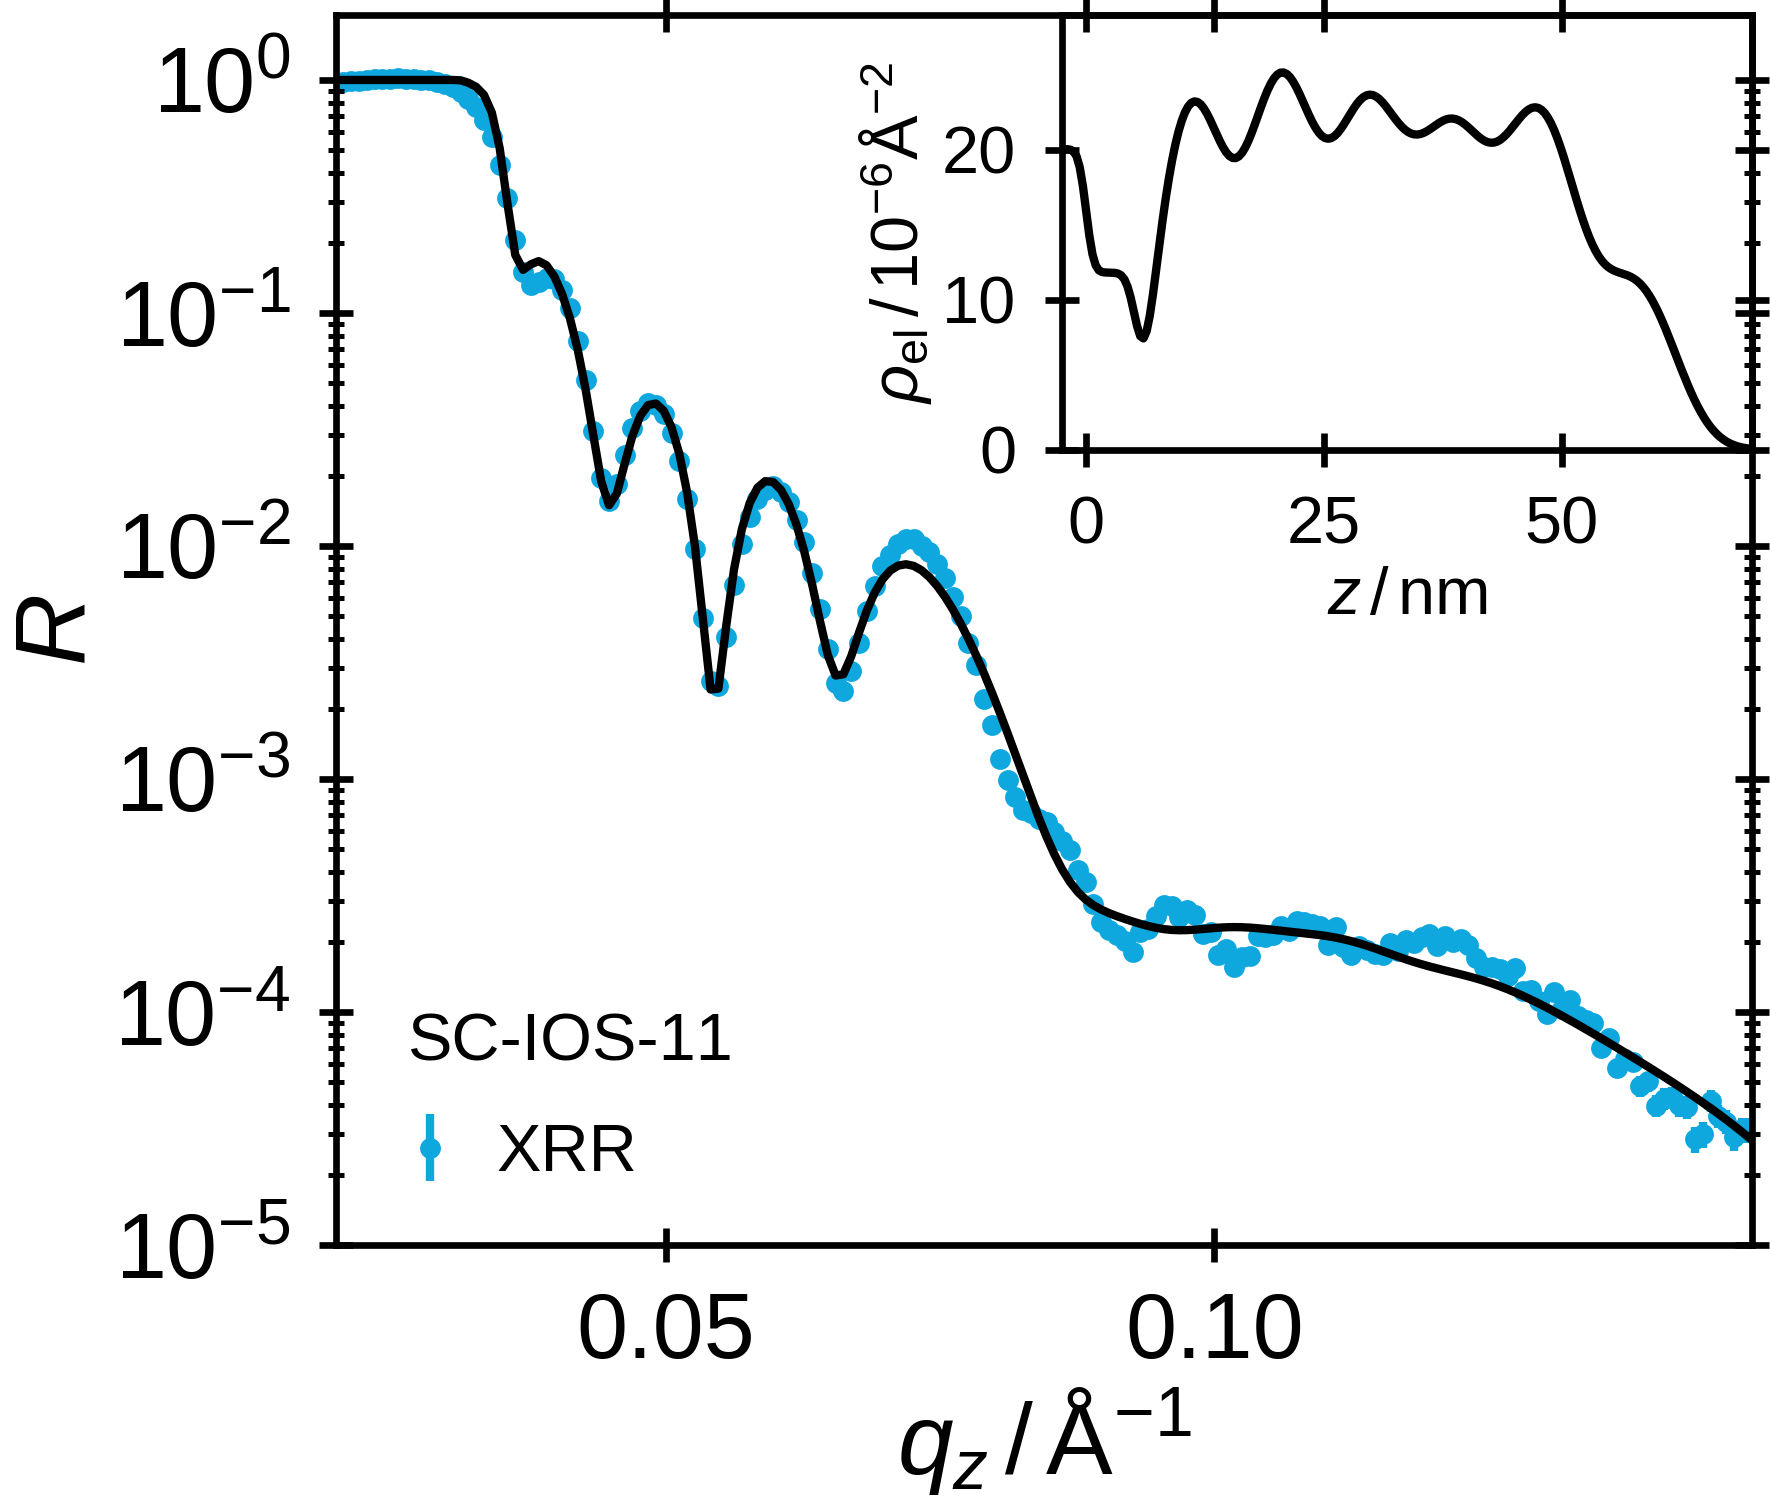
\includegraphics{looselyPackedNP_VerticalStructure_SC-IOS-11_XRR}
    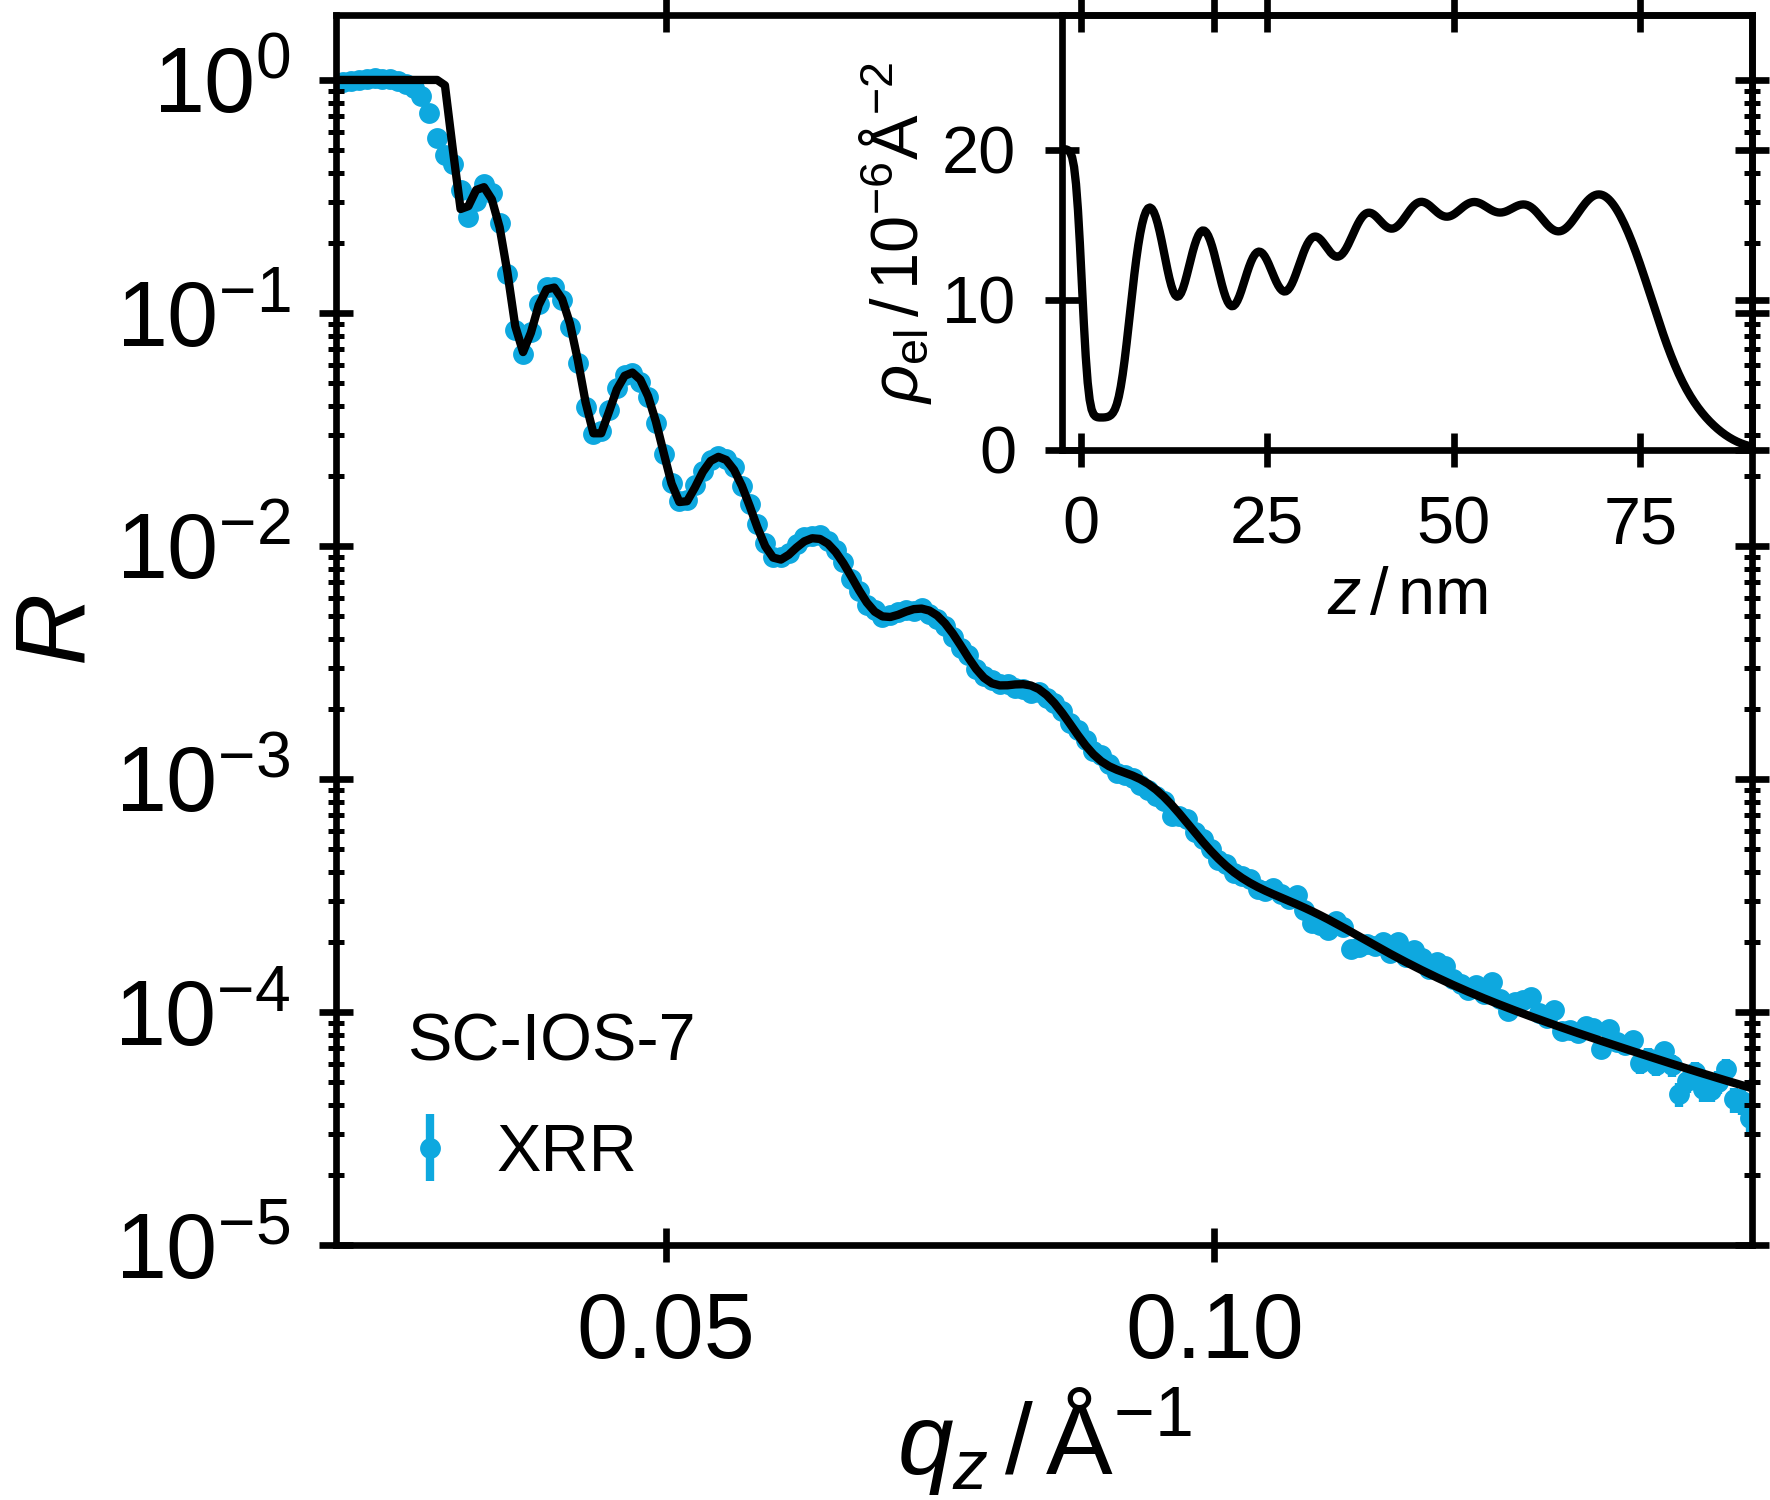
\includegraphics{looselyPackedNP_VerticalStructure_SC-IOS-7_XRR}
    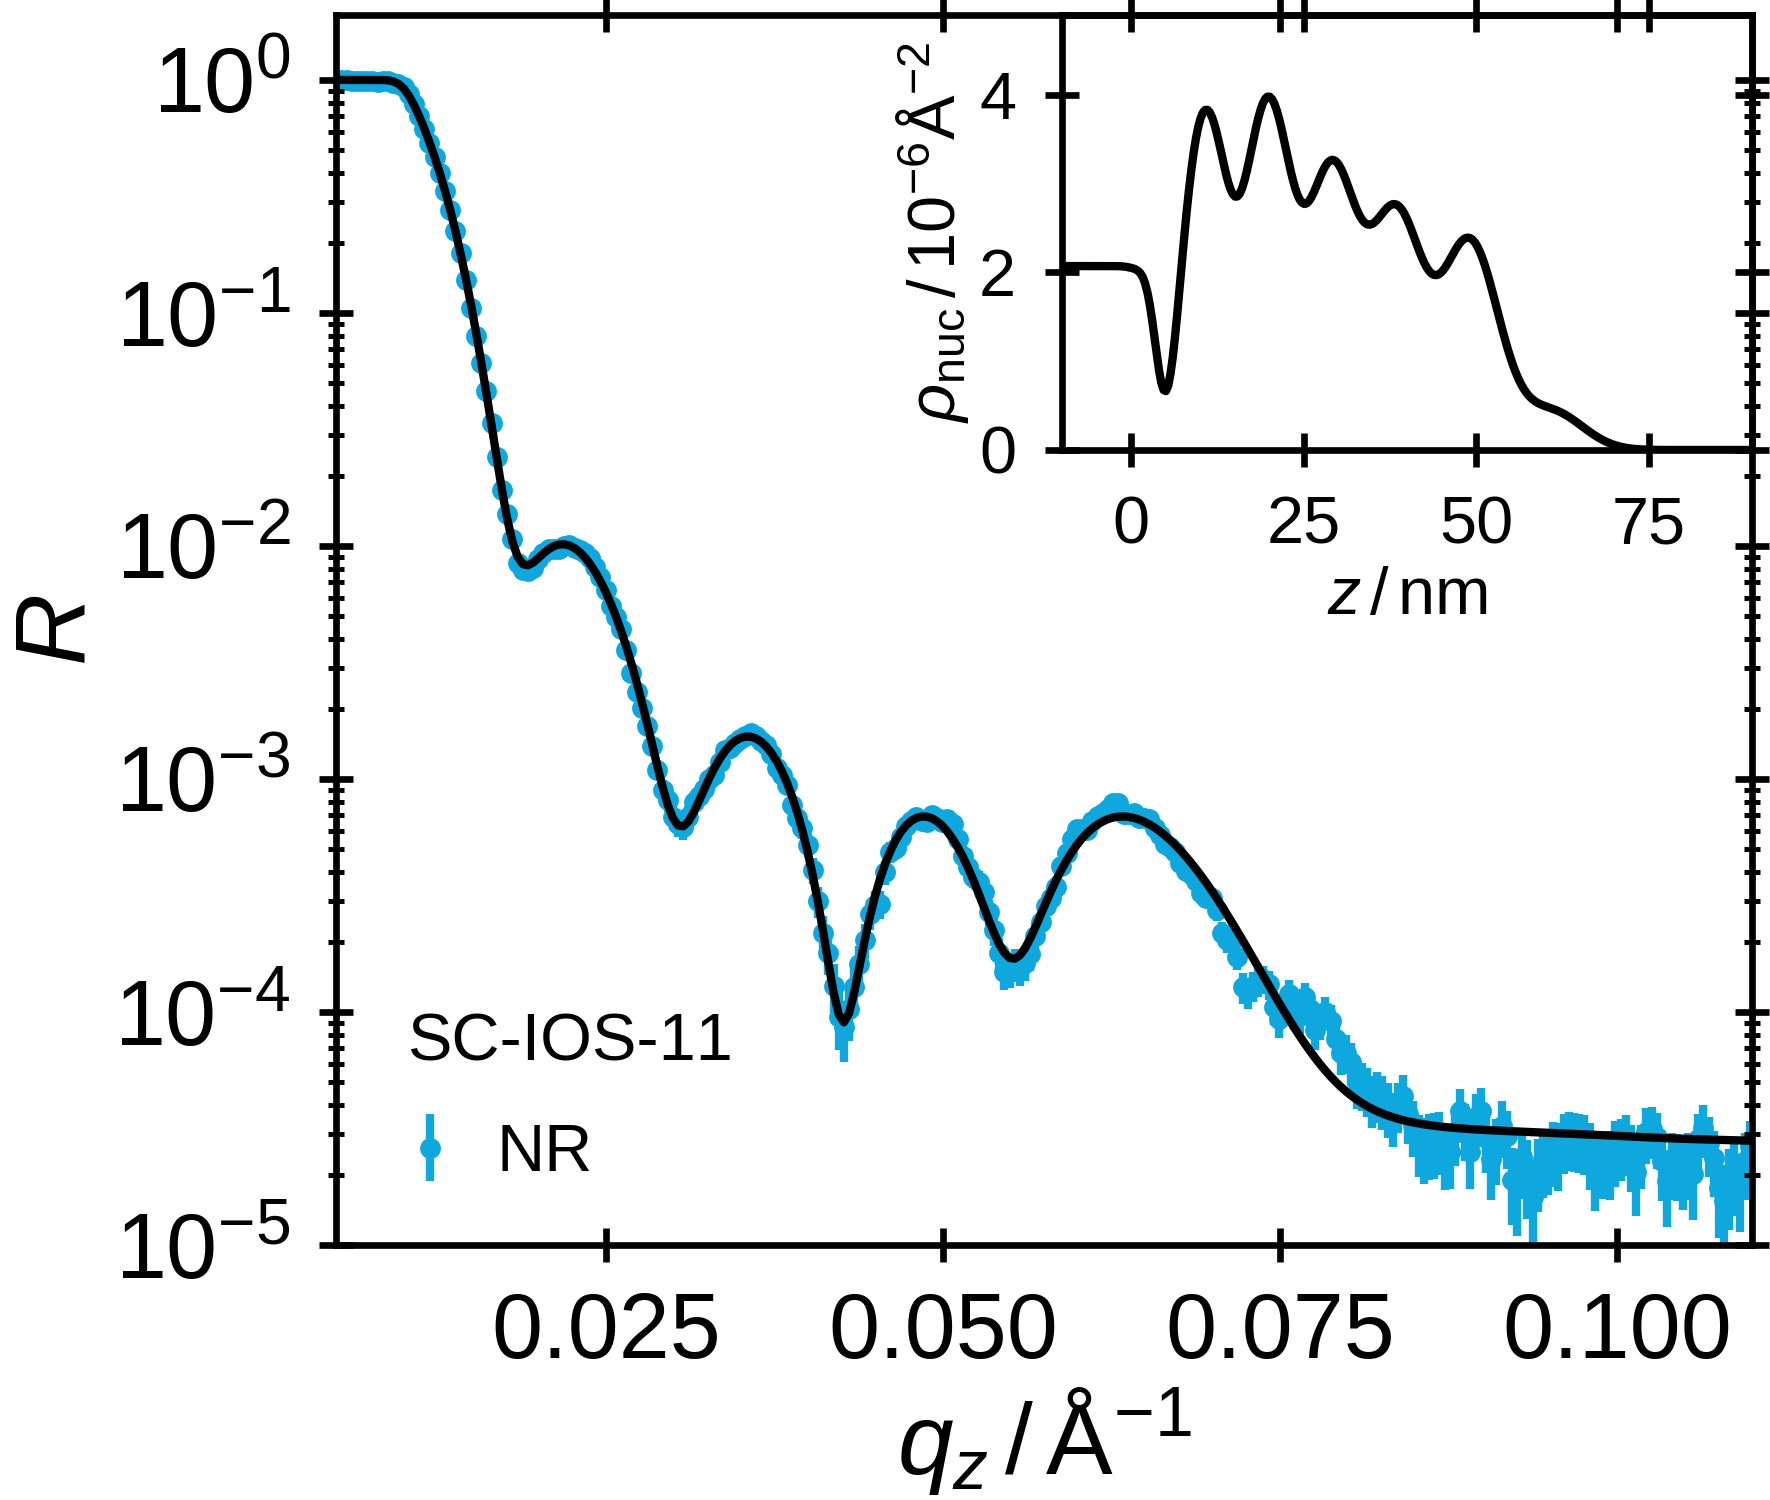
\includegraphics{looselyPackedNP_VerticalStructure_SC-IOS-11_PNR}
    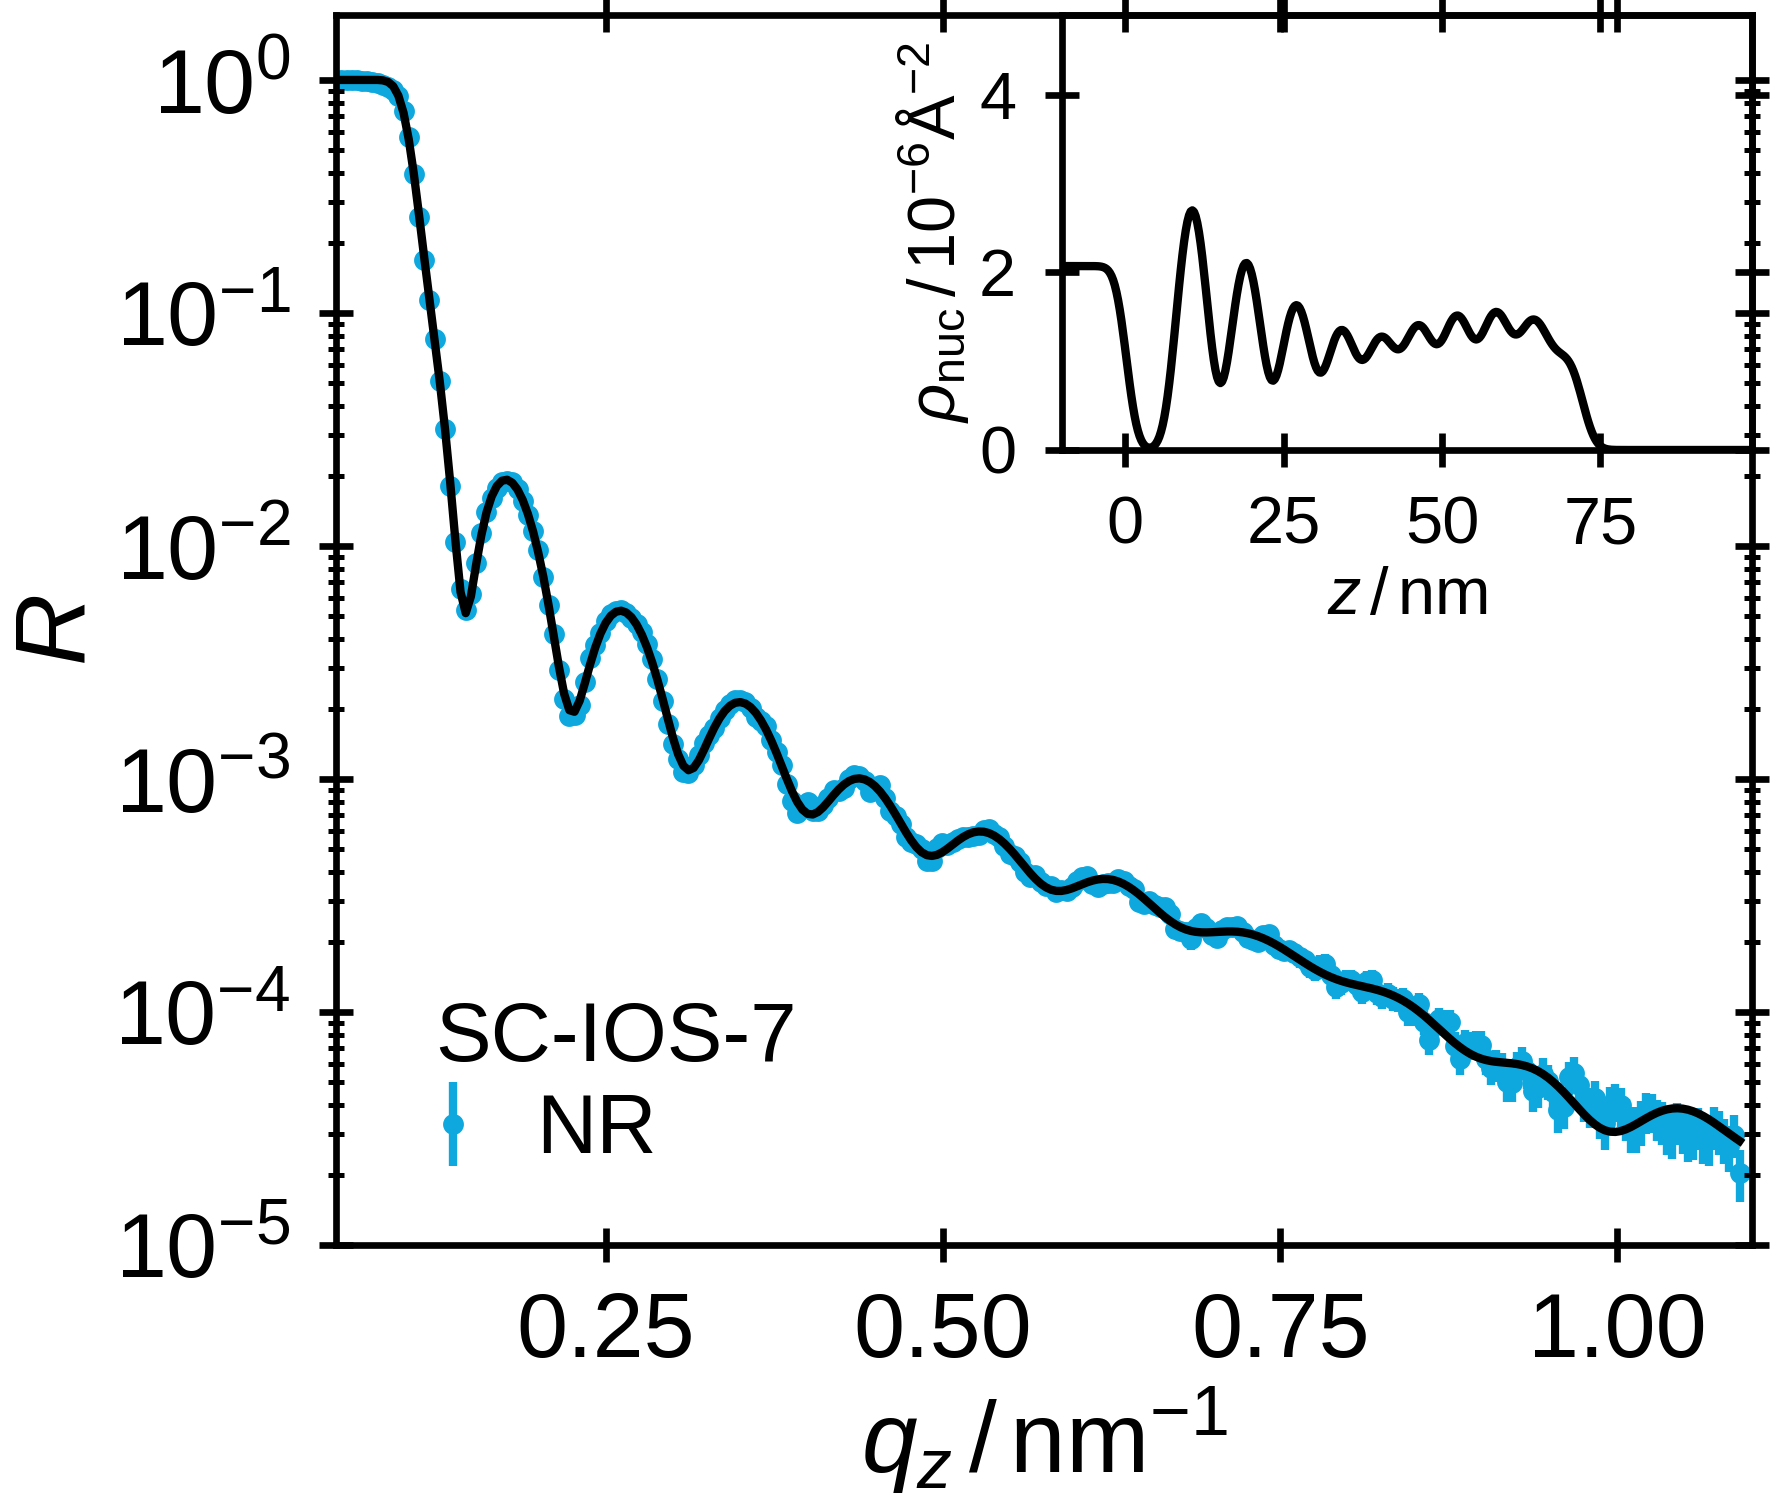
\includegraphics{looselyPackedNP_VerticalStructure_SC-IOS-7_PNR}
    \caption{\label{fig:looselyPackedNP:layer:reflectivity}X-ray (upper) and neutron (lower) reflectometry from SC-IOS-11 (left) and SC-IOS-7 (right). The insets shows the scattering length density model of the fitted reflectometry curve (black).}
  \end{figure}

  The electronic and nuclear structure of SC-IOS-11 and SC-IOS-7 is studied with depth-resolution using X-ray and neutron reflectometry at room temperature and ambient conditions.
  The X-ray reflectivity was measured on a Bruker D8 Advance and the neutron reflectivity has been measured on SuperADAM at the ILL (\refsec{ch:lss:superadam}).
  The reflectivity of both samples and both experiments is shown in \reffig{fig:looselyPackedNP:layer:reflectivity}.
  The reflectivity shows in all cases visible oscillations, which associate with the sample thickness.
  From the distance of the minima, the sample thickness is estimated to $52 \unit{nm}$ for SC-IOS-11 and $75 \unit{nm}$ for SC-IOS-7.
  % SC-IOS-11 shows additionally an visible increase of the reflectivity around $q \eq 0.63 \unit{\angstrom^{-1}}$, which correlates with the length scale of the nanosphere diameter of IOS-11 that is in the order of $10 \unit{nm}$.
  % For SC-IOS-7, the length scale of $7 \unit{nm}$ would expect a correlation peak in the order of $q \eq 0.9 \unit{\angstrom^{-1}}$, which is not visible from a qualitative evaluation.

  To quantitatively evaluate the reflectivity, a scattering length profile model is fitted, which assumes that the sample is compromised of multiple stacked spheres, which rest on a silicon substrate.
  Despite effort, it was not possible to fit both neutron and X-ray reflectometry with the same structural model and only varied scattering length density simultaneously for either of the two samples.
  There are various reasons as to why it is not possible to fit both datasets with the same model:
  For one the measurement of the same samples lie more than two years apart and the samples have both been exposed to cryogenic temperatures in an intermediate experiment before the XRR experiment has been performed.
  For the other, the neutron reflectivity experiments scans over a larger area of the sample due to the larger beam size and it's possible that the average density is obtained slightly differently in comparison to the x-ray reflectivity experiment due to the complex structure of the sample.
  Therefore, the layer density and layer packing fraction are varied independently for both experiments, yielding the scattering length density profiles shown in the insets of \reffig{fig:looselyPackedNP:layer:reflectivity} that are parameterized by the values given in \reftab{tab:looselyPackedNP:layers:reflectivity}.

  The calculated reflectivities are able to reproduce most of the characteristics of the experimental reflectivity curves.
  Deviations are visible in the X-ray reflectivity in both cases.
  For SC-IOS-11 the high q-range above $1.5 \unit{\angstrom^{-1}}$ is not properly described, which hints to features in the scattering length density that are missed on the length scale below $4 \unit{nm}$.
  For SC-IOS-7 on the other hand, the critical edge is smaller than the edge calculated for a silicon substrate and therefore a discrepancy is visible here.
  The formulated models do not account for absorption due to the nanoparticle layer, which would decrease the critical edge and therefore and becomes visible in this case.

  \begin{table}[!htbp]
    \centering
    \caption{\label{tab:looselyPackedNP:layers:reflectivity}Parameters for the layer of multiple nanospheres shown in \reffig{fig:looselyPackedNP:layer:reflectivity}. The parameters $\eta$ are the two dimensional packing density for each layer and $\Delta z$ are the shifts of the layer center from the pitch $\sqrt{8/3} (R+D_\mathrm{OA}$). The other parameters are the thickness of the spacer layer on the substrate $d_\mathrm{spacer}$, its SLD $\rho_\mathrm{spacer}$, the substrate roughness $\sigma$, the rate of roughness increase with layer height $\Delta \sigma$, and the wavelength spread of the instrument $\sigma_\lambda / \lambda$. The nanosphere parameters are fixed as determined from SAS (\refsec{sec:looselyPackedNS:nanoparticle:sas}).}
    \begin{tabular}{ c | l | l | l | l}
      \rule{0pt}{2ex} \textbf{Reflectometry}  & \multicolumn{2}{c}{\textbf{SC-IOS-11}} & \multicolumn{2}{c}{\textbf{SC-IOS-7}} \\
      \rule{0pt}{2ex}                   & XRR       & NR        & XRR       & NR \\
      \hline
       $\eta_1     \, / \unit{\%}$      & $65(1)$   & $96(1)$   & $63(6)$   & $99.2(1)$\\
       $\eta_2     \, / \unit{\%}$      & $88(1)$   & $103(1)$  & $68(9)$   & $77.4(1)$\\
       $\eta_3     \, / \unit{\%}$      & $87(1)$   & $89(1)$   & $72(11)$  & $59.8(1)$\\
       $\eta_4     \, / \unit{\%}$      & $80(1)$   & $79(1)$   & $65(19)$  & $49.0(1)$\\
       $\eta_5     \, / \unit{\%}$      & $73(1)$   & $78(1)$   & $57(31)$  & $45.4(1)$\\
       $\eta_6     \, / \unit{\%}$      & $17(1)$   & $18(1)$   & $71(29)$  & $50.0(1)$\\
       $\eta_7     \, / \unit{\%}$      &           &           & $87(18)$  & $54.1(1)$\\
       $\eta_8     \, / \unit{\%}$      &           &           & $97(15)$  & $55.2(1)$\\
       $\eta_9     \, / \unit{\%}$      &           &           & $22(21)$  & $51.2(1)$\\
       $\eta_{10}     \, / \unit{\%}$   &           &           & $76(42)$  & $35.4(2)$\\
       \hline
       $\Delta z_1 \, / \unit{nm} $     & $-1.6(1)$ & $-2.2(1)$ & $-0.8(2)$ & $-0.9(1)$\\
       $\Delta z_2 \, / \unit{nm} $     & $-3.4(1)$ & $-2.8(1)$ & $-0.9(2)$ & $-0.0(1)$\\
       $\Delta z_3 \, / \unit{nm} $     & $-3.0(1)$ & $-2.6(1)$ & $-0.9(2)$ & $-0.6(1)$\\
       $\Delta z_4 \, / \unit{nm} $     & $-3.4(1)$ & $-2.6(1)$ & $-1.1(4)$ & $-1.5(1)$\\
       $\Delta z_5 \, / \unit{nm} $     & $-3.1(1)$ & $-1.5(1)$ & $-0.8(6)$ & $-2.3(1)$\\
       $\Delta z_6 \, / \unit{nm} $     & $-2.1(1)$ & $-0.2(1)$ & $-0.7(8)$ & $-2.5(1)$\\
       $\Delta z_7 \, / \unit{nm} $     &           &           & $-1.2(5)$ & $-2.4(1)$\\
       $\Delta z_8 \, / \unit{nm} $     &           &           & $-1.5(5)$ & $-2.4(1)$\\
       $\Delta z_9 \, / \unit{nm} $     &           &           & $ 0(1)$   & $-2.6(1)$\\
       $\Delta z_{10} \, / \unit{nm} $  &           &           & $-1(2)$   & $-3.2(1)$\\
       \hline
       $d_\mathrm{spacer}   \, / \unit{nm} $                        & $5.15(3)$ & $5.0(1)$  & $5.3(1)$ & $6.1(1)$\\
       $\rho_\mathrm{spacer}\, / \unit{10^{-6} \angstrom^{-2}} $    & $11.9(2)$ & $1.3(1)$  & $2(1)$   & $0.0(1)$\\
       $\sigma     \, / \unit{nm} $                                 & $0.47(3)$ & $0.6(5)$  & $0.62(2)$& $1.45(6)$\\
       $\Delta \sigma$                                              & $0.006(2)$& $0.051(2)$& $0.037(1)$ & $0(0)$\\
       $\sigma_\lambda / \lambda\, / \unit{\%}$                     & $2.1(1)$  & $0.21$    & $2.1(1)$  & $0.21$\\
       $\sigma_\theta \, / \unit{mrad}$                             & $0$       & $0.3$     & $0$       & $0.3$ \\
       \hline
      %  $R               \, / \unit{nm}$                               & \multicolumn{2}{c}{$3.8$}  & \multicolumn{2}{c}{$0$} \\
      %  $D_\mathrm{shell}\, / \unit{nm}$                               & \multicolumn{2}{c}{$1.6$}  & \multicolumn{2}{c}{$3.54$} \\
      %  $D_\mathrm{OA}   \, / \unit{nm}$                               & \multicolumn{2}{c}{$1.82$} & \multicolumn{2}{c}{$1.69$} \\
      %  $\sigma_R        \, / \unit{\%}$                               & \multicolumn{2}{c}{$5.45$} & \multicolumn{2}{c}{$7.52$} \\
       $\rho_\mathrm{core}\, / \unit{10^{-6} \angstrom^{-2}}      $   & $44.3$  & $8.340$ & $44.3$ & $8.340$\\
       $\rho_\mathrm{shell}\, / \unit{10^{-6} \angstrom^{-2}}      $  & $40.5$  & $7.000$ & $40.5$ & $7.000$\\
       $\rho_\mathrm{OA}\, / \unit{10^{-6} \angstrom^{-2}}     $      & $8.52$  & $0.078$ & $8.52$ & $0.078$\\
       $\rho_\mathrm{substrate}\, / \unit{10^{-6} \angstrom^{-2}} $   & $20.1$  & $2.072$ & $20.1$ & $2.072$\\
      \hline
    \end{tabular}
  \end{table}
  The two dimensional packing fractions $\eta$ are in the order of $80 \unit{\%}$ for the five layers and $18 \unit{\%}$ for the upper layer.
  $\Delta z$ is in all cases negative in the order of $1 - 3 \unit{nm}$.
  For SC-IOS-7 the same observation in $\Delta z$ can be made and the packing fraction $\eta$ are lower being in an order of magnitude of $50 - 70 \unit{\%}$.
  For both samples, a spacer layer between the nanospheres and the silicon is resolved with approximately $5 \unit{nm}$ size.
  The base roughness of the sample is in the order of $0.5 - 1.5 \unit{nm}$ at the substrate and shows, if at all, a small increase with a slope in the order of $0.04 \unit{nm / nm}$ with respect to the layer height.
  The fitted roughness parameter is to be understood in this context as a model of the spread in the respective layer positions across the measured area within the reflectivity experiment.
  The increasing roughness with layer height is therefore to be understood as a larger uncertainty in the positions of the specific layer across the sample.

  The parameters of the sphere layer positions and their respective layer packing density are transformed to a depiction in \reffig{fig:looselyPackedNP:layer:reflectivityDepiction} for each experiment.
  Here, the two-dimensional packing fraction $\eta$ are translated into an average particle distance in the layer by
  \begin{align}
    r_\mathrm{pp} \eq \sqrt{\frac{\eta_\mathrm{CP}}{\eta}} 2 (R + D_\mathrm{shell} + D_\mathrm{OA}),
  \end{align}
  where $\eta_\mathrm{CP}$ is the dense circle packing fraction given by $\eta_\mathrm{CP} \eq \pi / \sqrt{12} \approx 90.7 \%$.
  From the depiction it becomes visible for IOS-SC-11 that the negative shift $\Delta z$ from the calculated pitch correlates with the lowered lateral packing density as the layers are merged by their oleic acid shells in all cases slightly into each other.
  The illustration also shows clearer that for IOS-SC-7 the obtained scattering length density profiles show both for X-ray and neutron reflectivity a less compact packing in the bulk of the sample.

  \begin{figure}[tb]
    \centering
    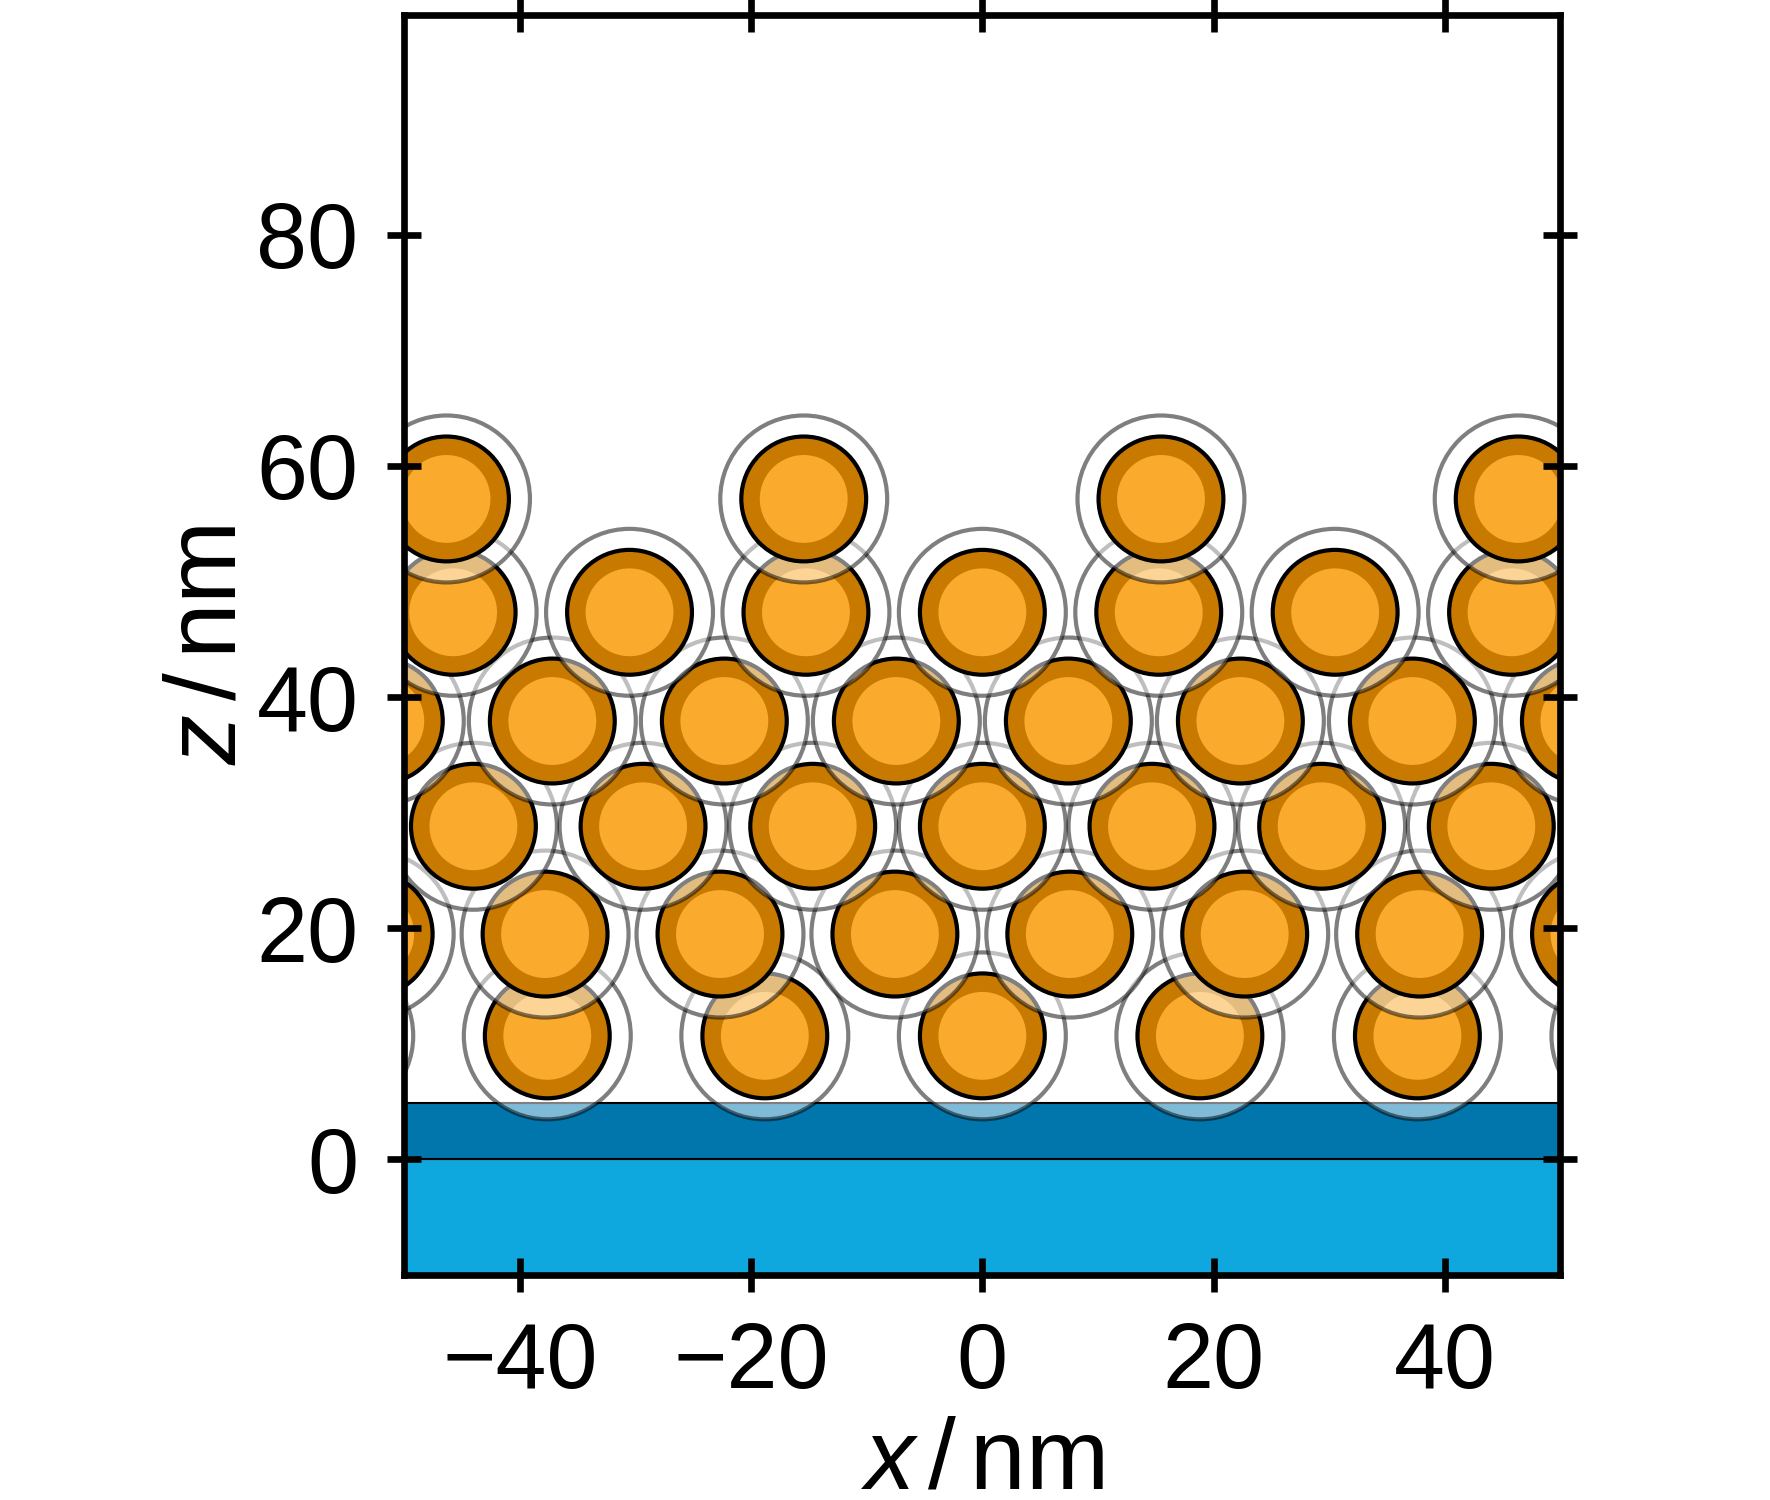
\includegraphics{looselyPackedNP_VerticalStructure_SC-IOS-11_XRRDepiction}
    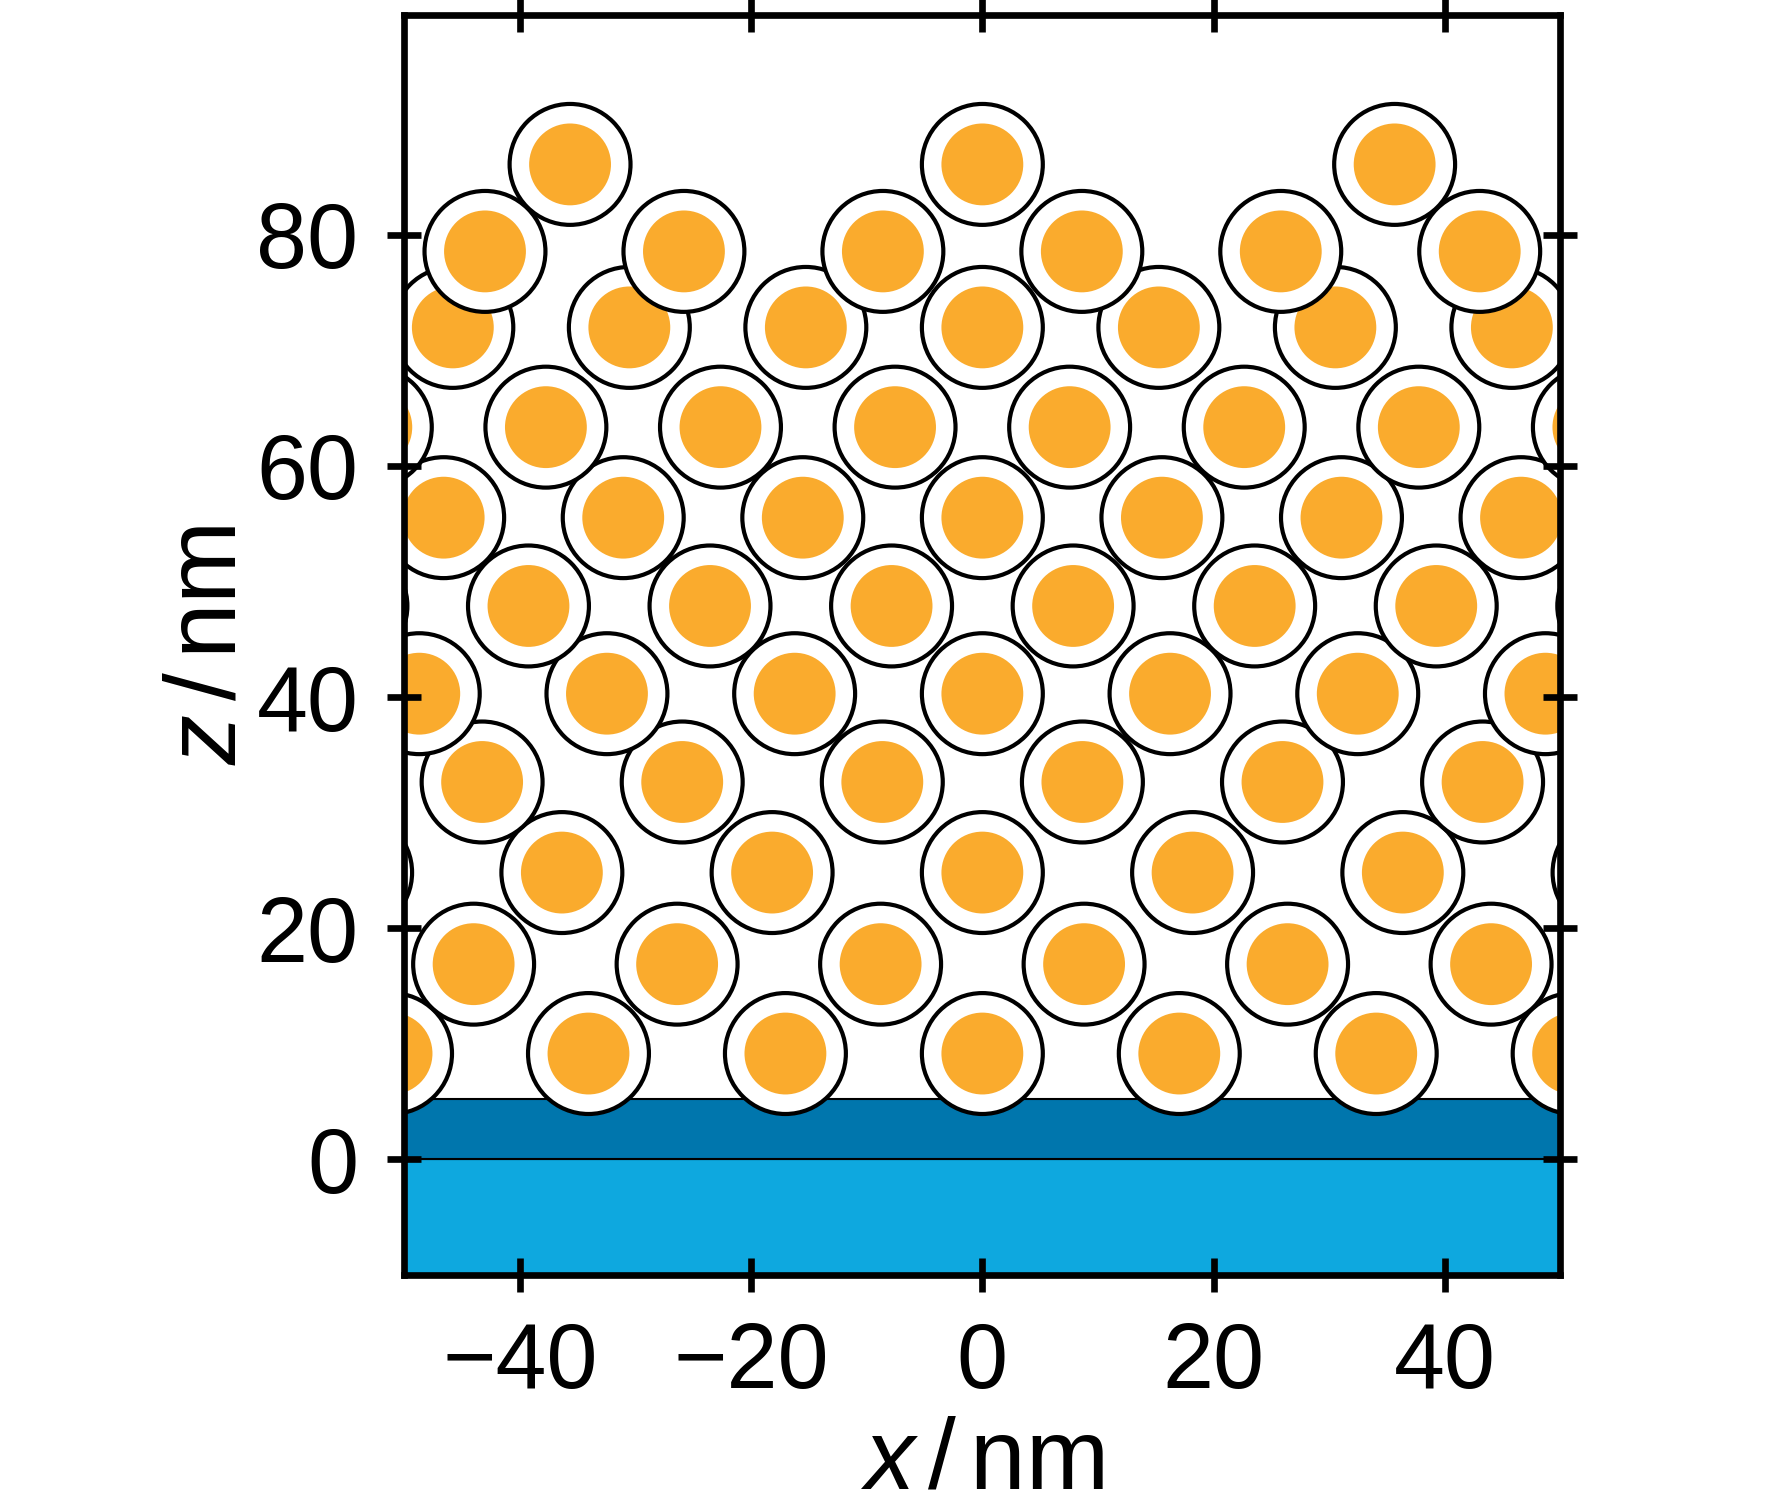
\includegraphics{looselyPackedNP_VerticalStructure_SC-IOS-7_XRRDepiction}
    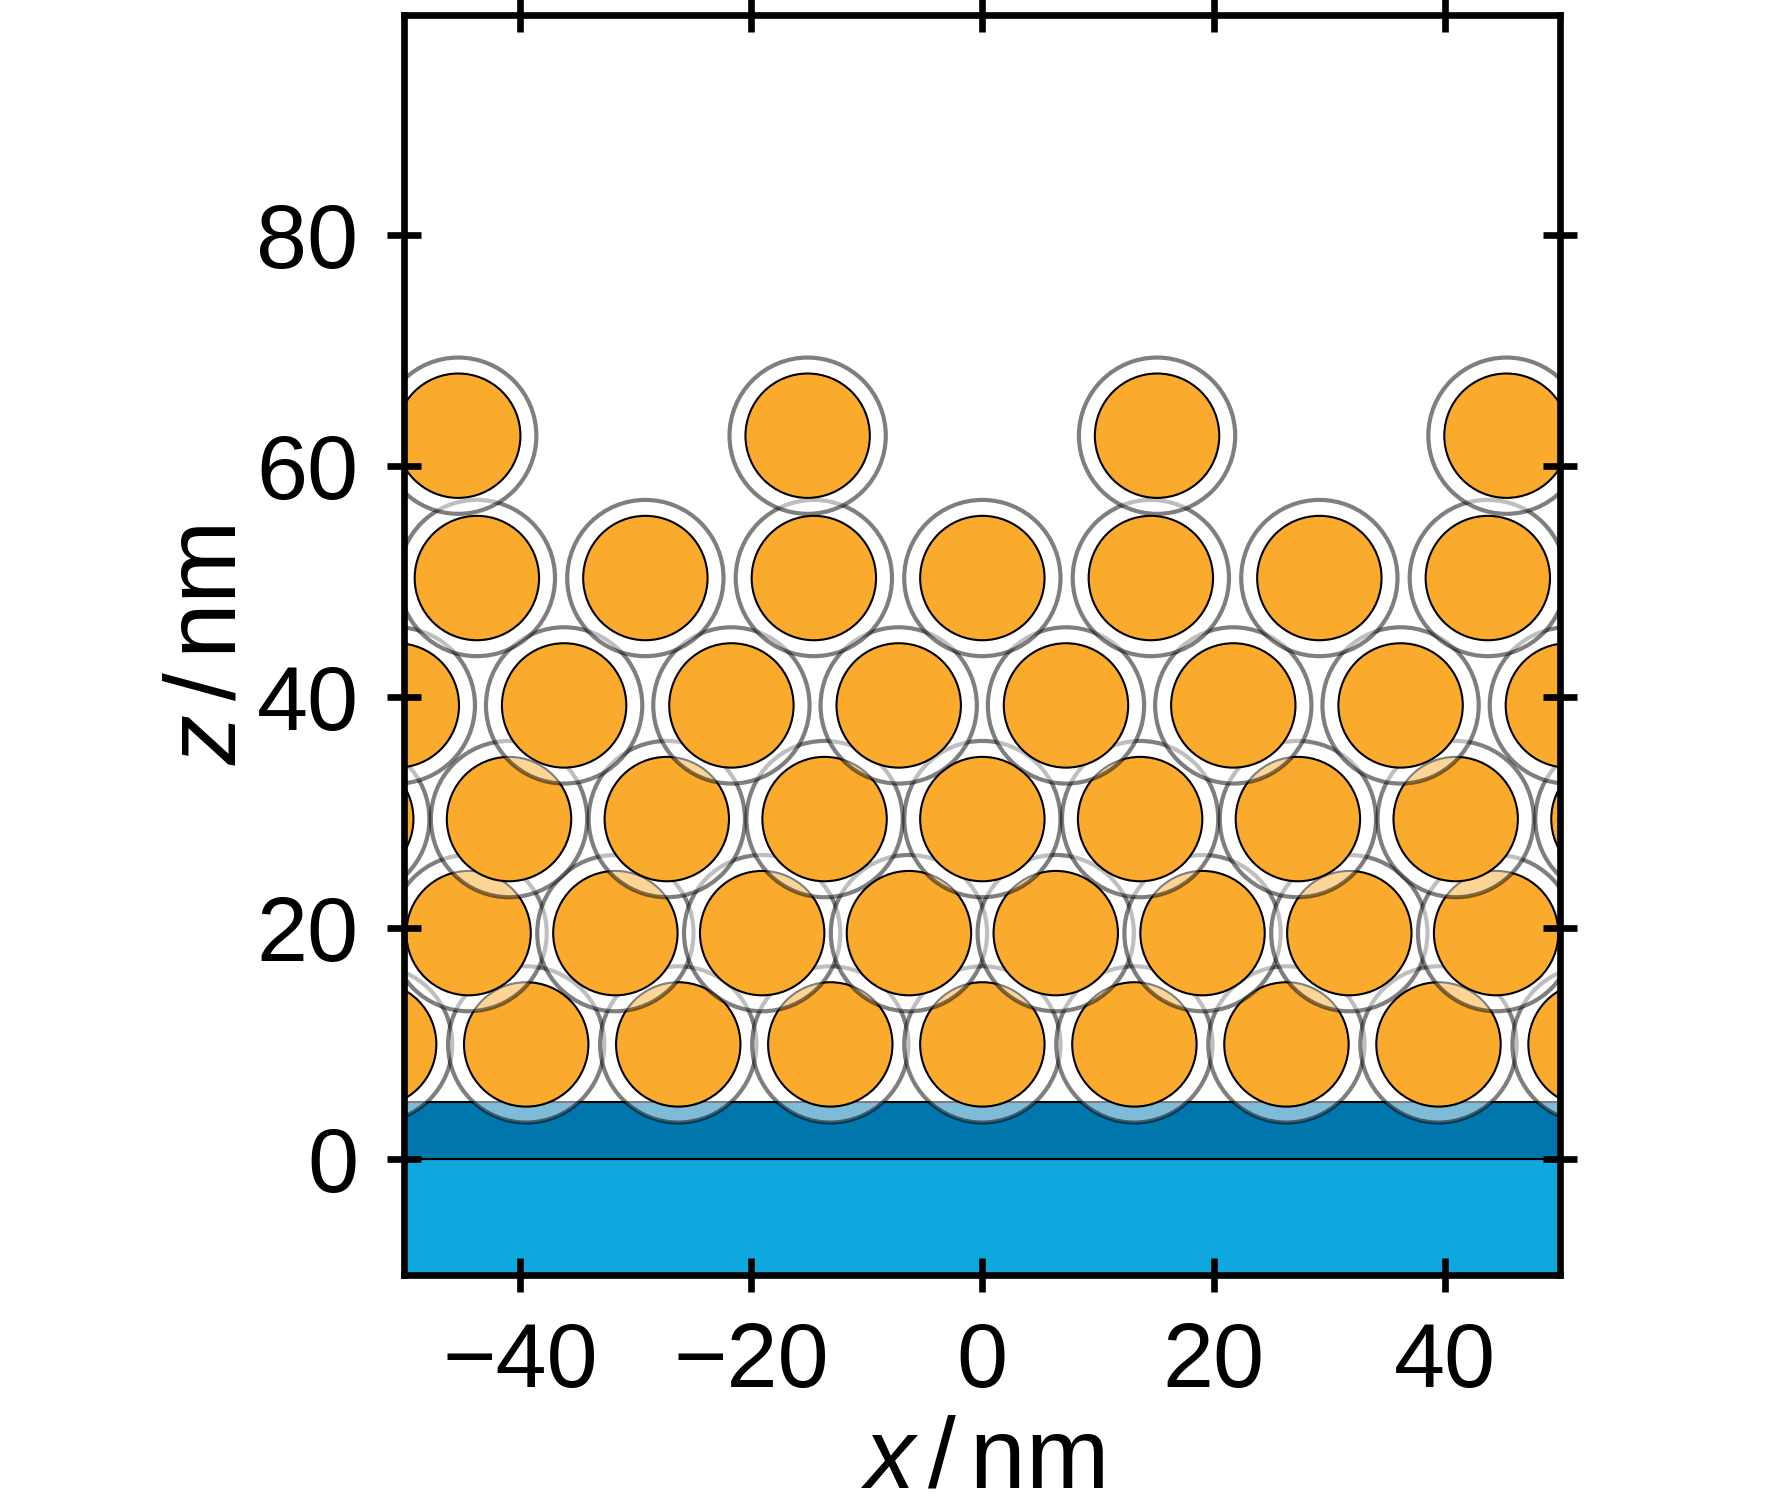
\includegraphics{looselyPackedNP_VerticalStructure_SC-IOS-11_PNRDepiction}
    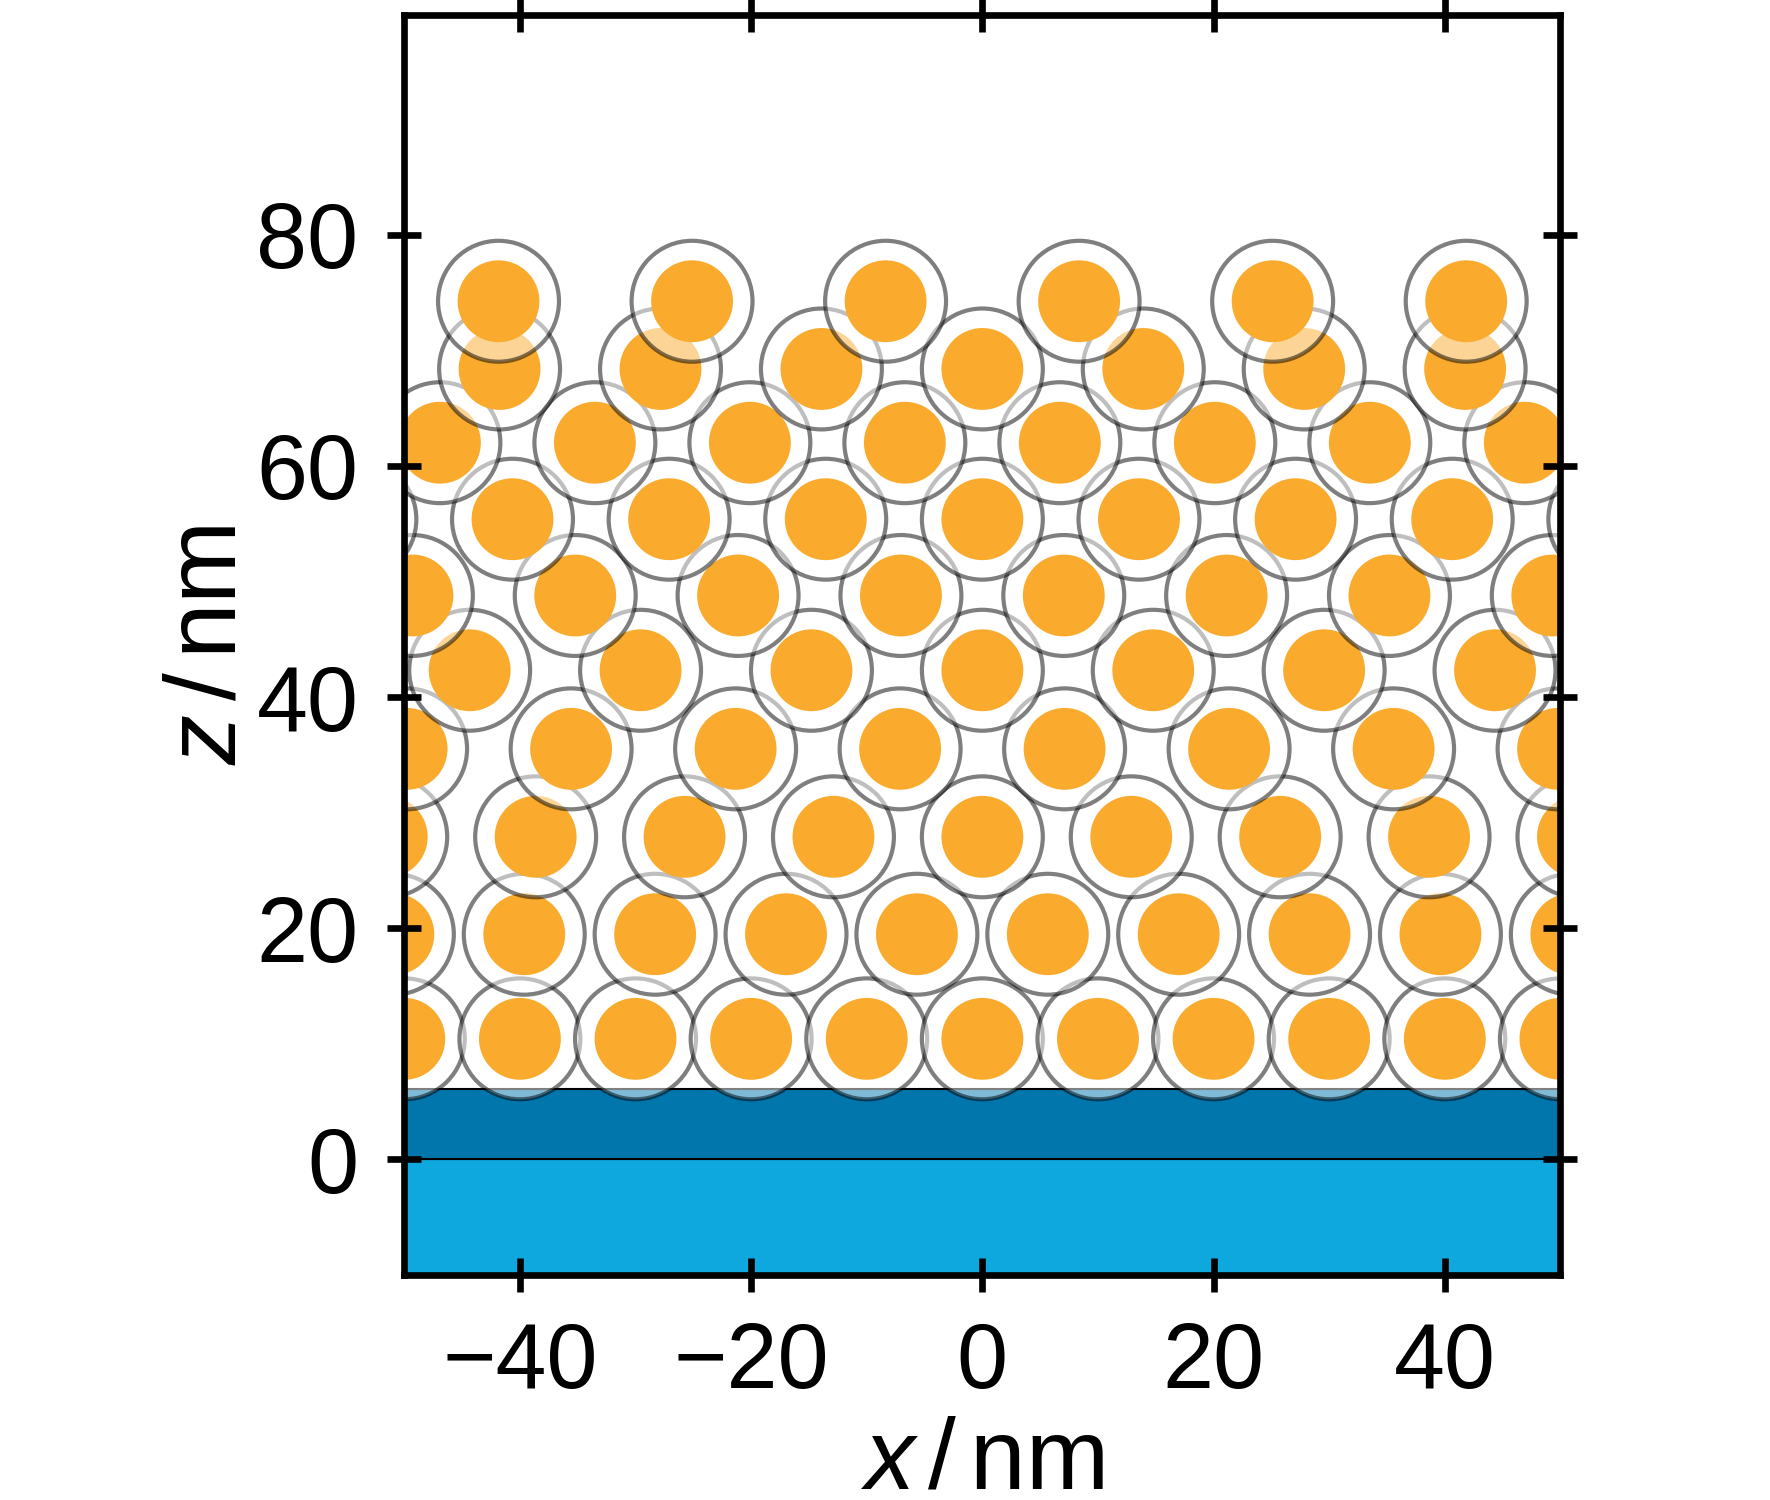
\includegraphics{looselyPackedNP_VerticalStructure_SC-IOS-7_PNRDepiction}
    \caption{\label{fig:looselyPackedNP:layer:reflectivityDepiction}Depiction of the fitted layer shifts $\Delta z$ and packing densities $\eta_i$ in \reftab{tab:looselyPackedNP:layers:reflectivity} showing the average structure of SC-IOS-11 (left) and SC-IOS-7 (right) as seen by X-ray reflectometry (upper) and neutron reflectometry (lower).}
  \end{figure}

  \begin{figure}[tb]
    \centering
    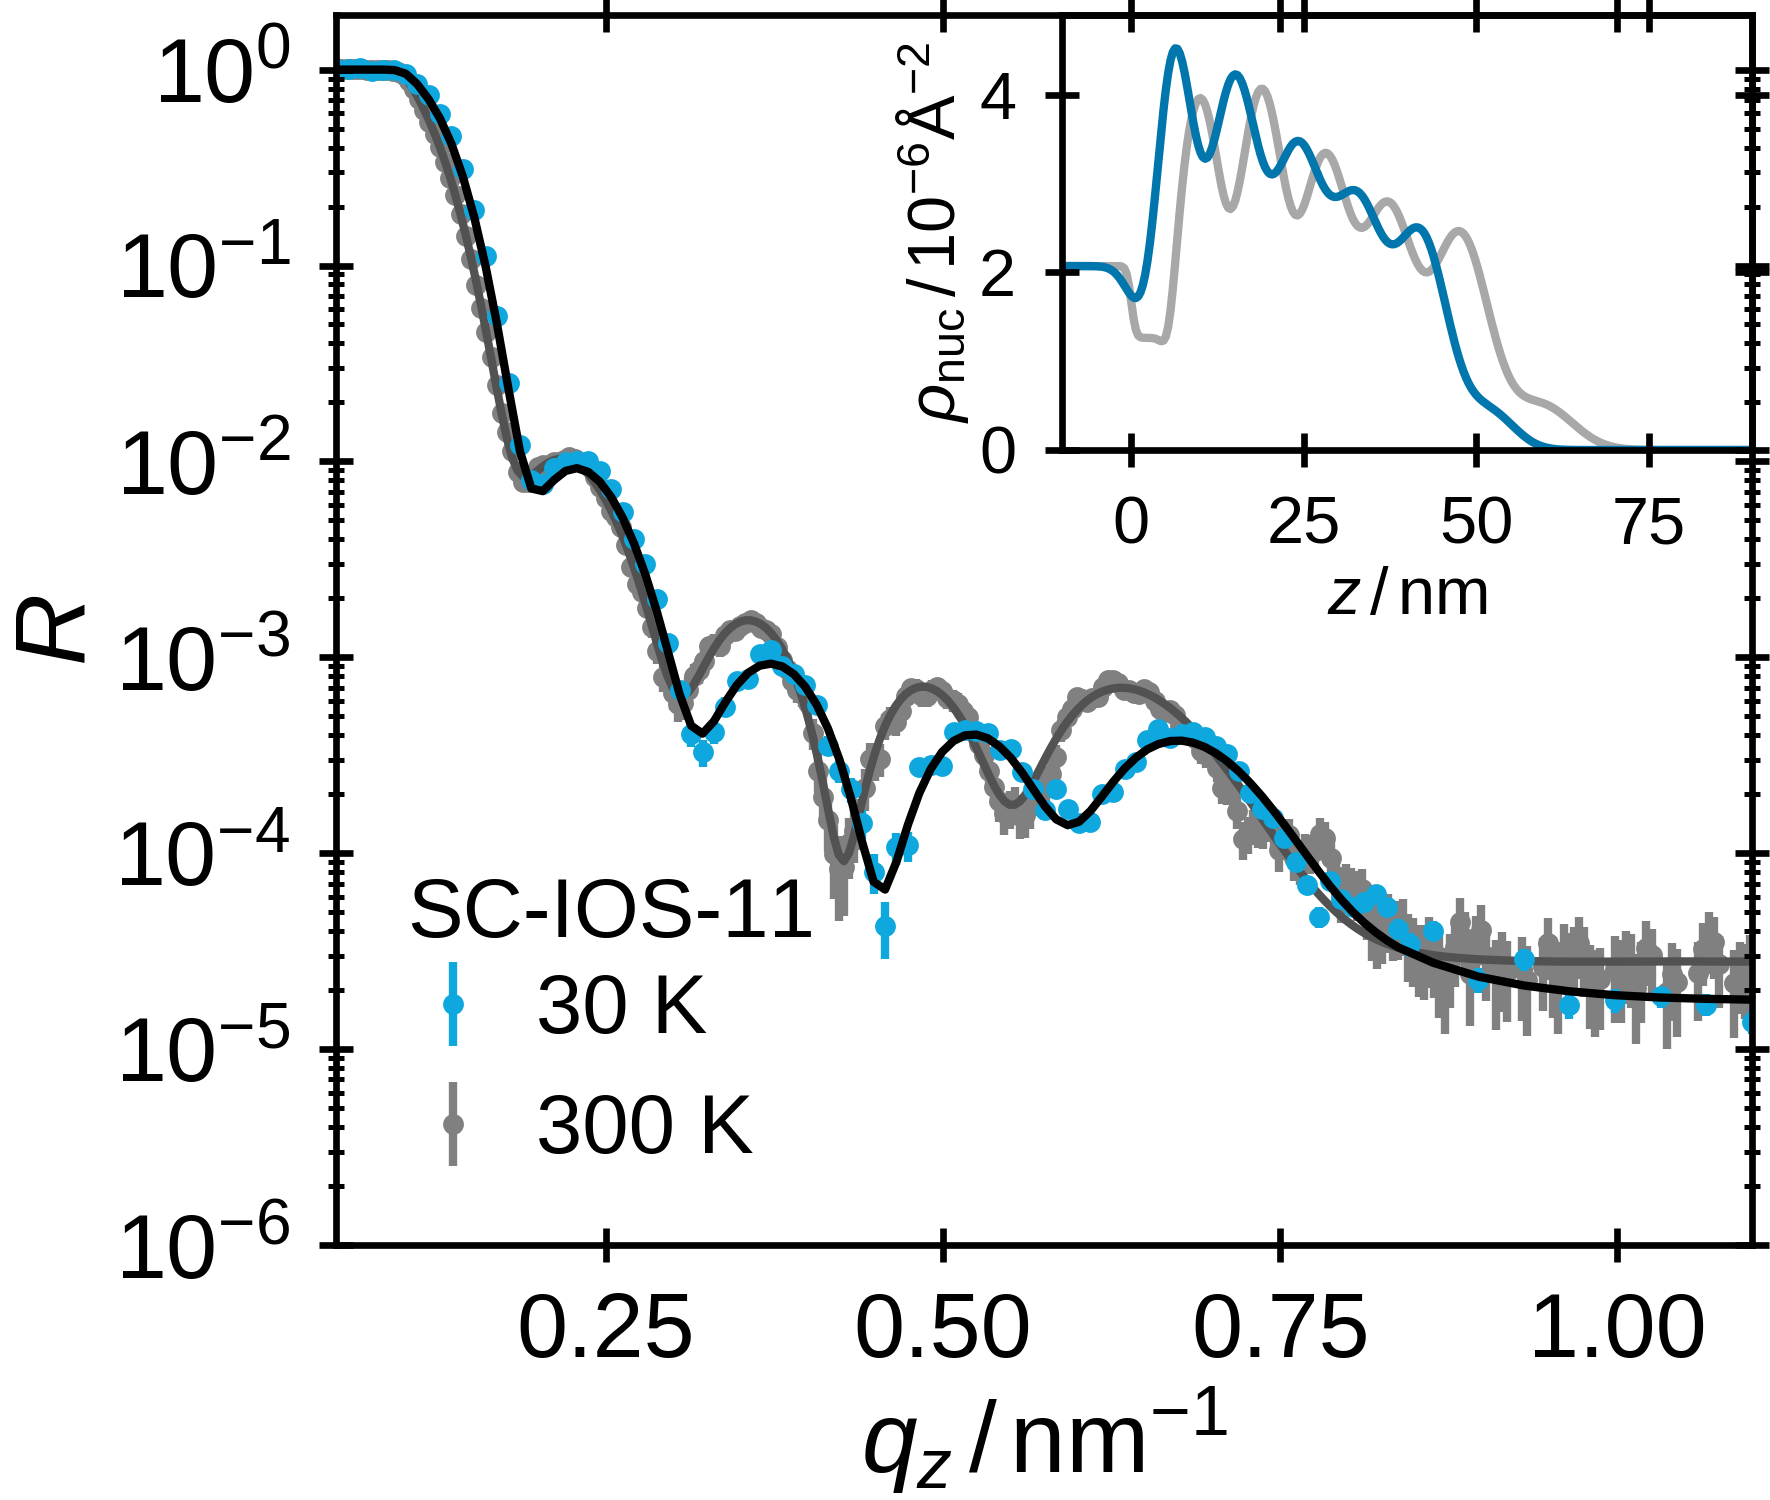
\includegraphics{looselyPackedNP_VerticalStructure_SC-IOS-11_PNR_Compare30K300K}
    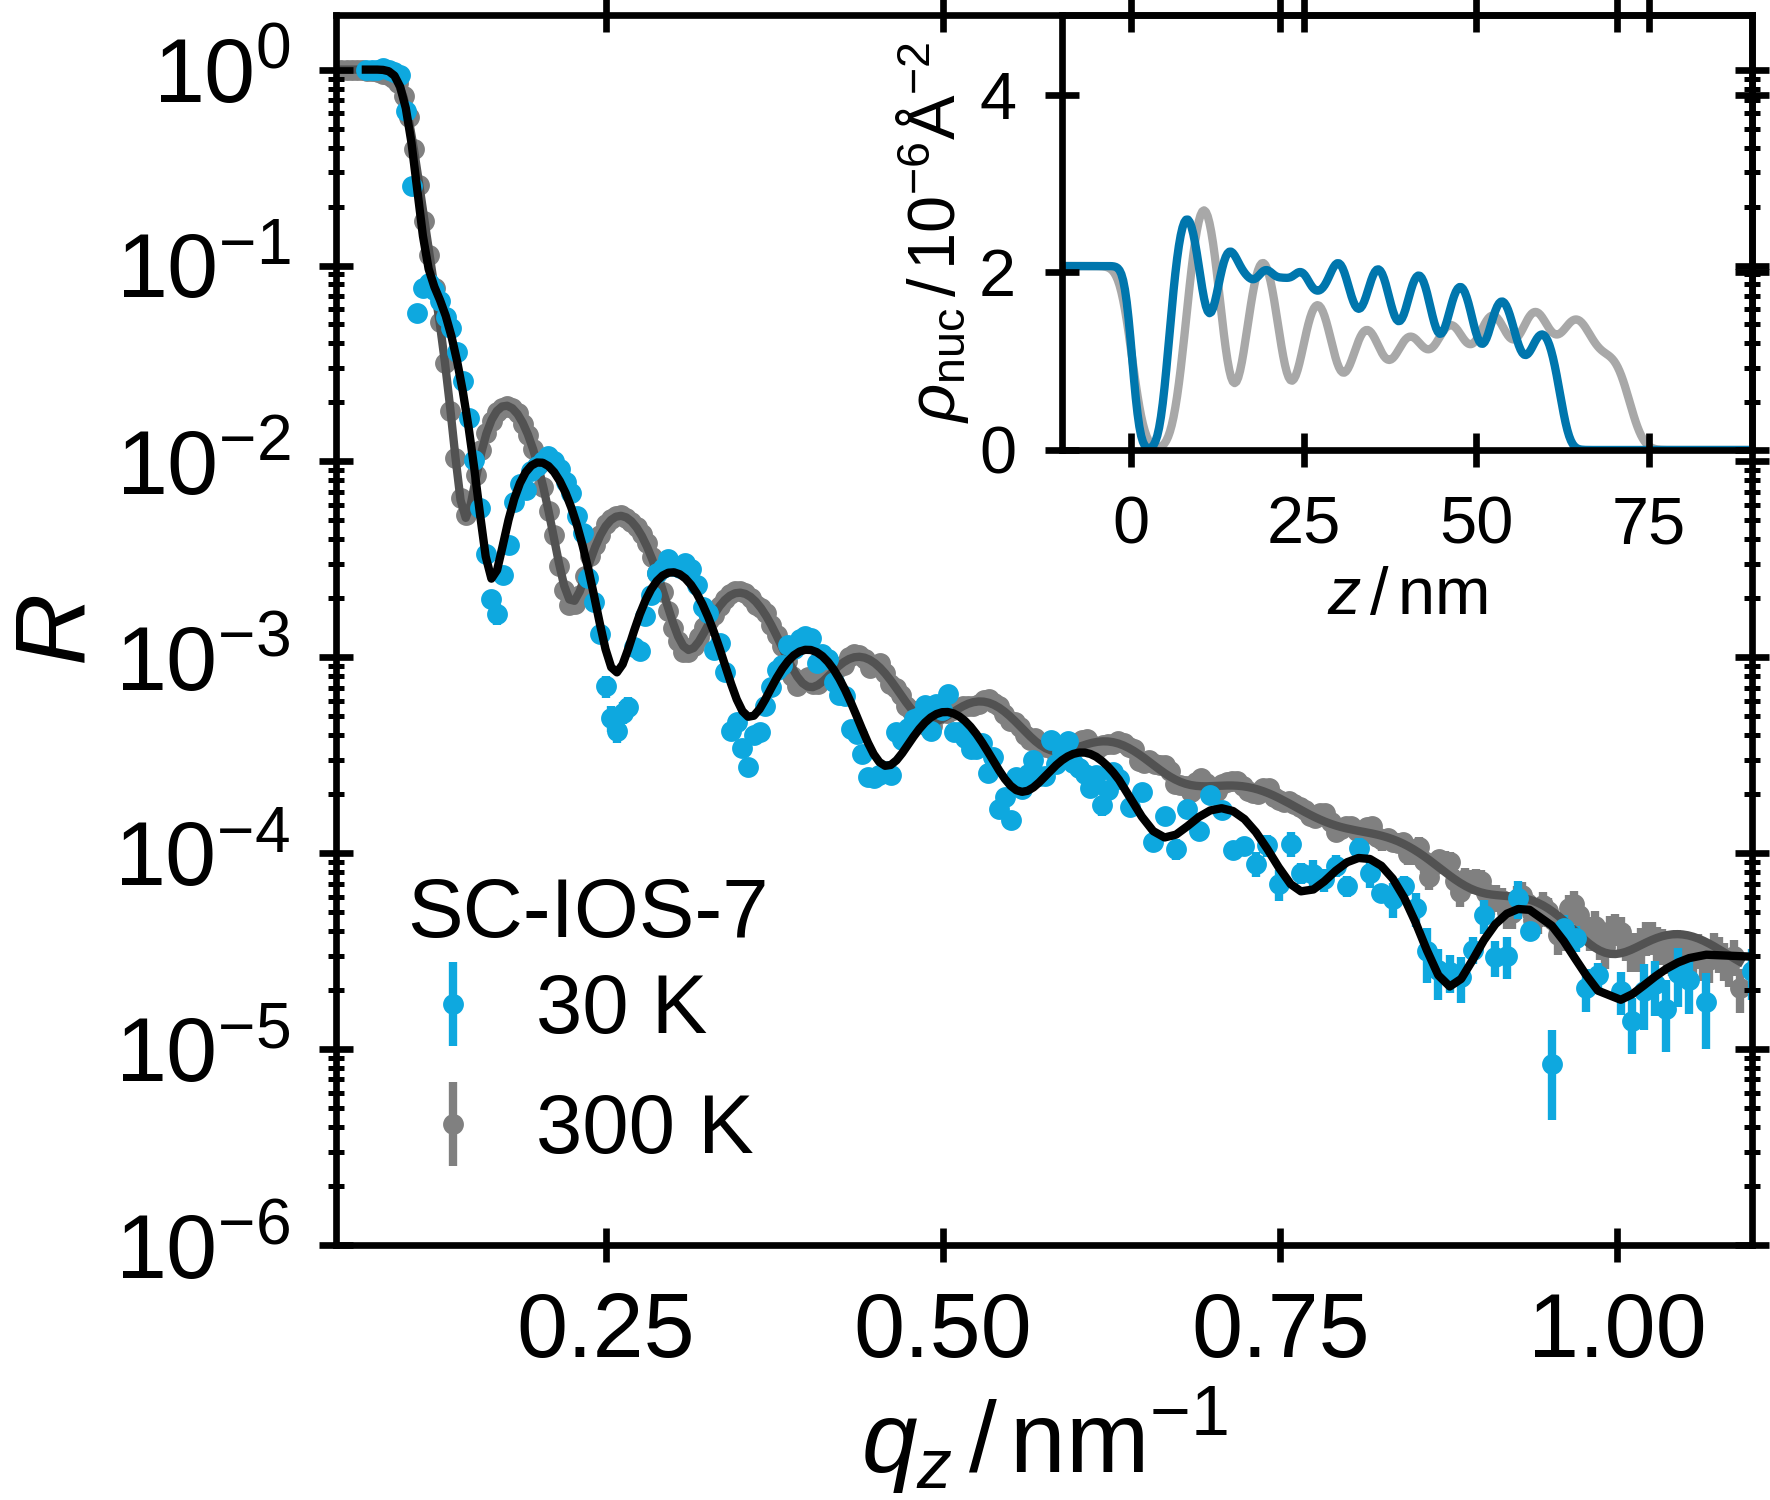
\includegraphics{looselyPackedNP_VerticalStructure_SC-IOS-7_PNR_Compare30K300K}
    \caption{\label{fig:looselyPackedNP:layer:pnrCompare30K300K}Comparison of 30 K and 300 K measurement of SC-IOS-11 (left) and SC-IOS-7 (right).}
  \end{figure}
  Additionally, neutron reflectometry has also been used to study the magnetic nanospheres at a lower temperature of $30 \unit{K}$.
  In \reffig{fig:looselyPackedNP:layer:pnrCompare30K300K}, the comparison of the reflectometry curves obtained at $30 \unit{K}$ and $300 \unit{K}$ is shown.
  A striking difference is that the low-temperature curves are in both cases shifted towards larger $q$ values.
  This translates to a compressed layer structure, which can be seen in the insets respectively, with the tabulated parameters in \reftab{tab:looselyPackedNP:layers:reflectivity30K}.
  Comparing the obtained shifts with the values at room temperature in \reftab{tab:looselyPackedNP:layers:reflectivity}, the nanoparticles have shifted $0.5 - 1.5 \unit{nm}$ closer to each other and slightly increased their packing density at low temperatures.
  The oleic acid coatings in the packing therefore seem to allow still some greater flexibility in the nanoparticle positions, which allowed upon freezing for the nanoparticles to get closer to one another.

  The here obtained scattering length density profiles are crucial for the evaluation of the spin density in the nanoparticle layers.
  As the presented formulation implements the small-angle scattering result for the nanoparticle size and composition by design correctly, they allow by evaluation of the polarized neutron reflectivities a direct comparison of the single nanoparticle to the layer magnetic properties in the following section.

  \begin{table}[!htbp]
    \centering
    \caption{\label{tab:looselyPackedNP:layers:reflectivity30K}Parameters for the layers measured with NR at $30 \unit{K}$. The layer packing density $\eta$ and the layer shifts $\Delta z$ are refit to adjust for the compressed sample.}
    \begin{tabular}{ c | l | l}
      \rule{0pt}{2ex} \textbf{NR @ 30 K}  & \textbf{SC-IOS-11} & \textbf{SC-IOS-7} \\
      \hline
       $\eta_1     \, / \unit{\%}$      & $111(9)$   & $86(27)$\\
       $\eta_2     \, / \unit{\%}$      & $112(2)$  & $73(16)$\\
       $\eta_3     \, / \unit{\%}$      & $96(1)$   & $65(15)$\\
       $\eta_4     \, / \unit{\%}$      & $85(2)$   & $65(20)$\\
       $\eta_5     \, / \unit{\%}$      & $83(5)$   & $69(21)$\\
       $\eta_6     \, / \unit{\%}$      & $20(3)$   & $66(16)$\\
       $\eta_7     \, / \unit{\%}$      &           & $65(14)$\\
       $\eta_8     \, / \unit{\%}$      &           & $60(11)$\\
       $\eta_9     \, / \unit{\%}$      &           & $55(9)$\\
       $\eta_{10}     \, / \unit{\%}$   &           & $43(7)$\\
       \hline
       $\Delta z_1 \, / \unit{nm} $     & $-4.1(3)$ & $-0.9(1)$\\
       $\Delta z_2 \, / \unit{nm} $     & $-2.9(3)$ & $-2.4(5)$\\
       $\Delta z_3 \, / \unit{nm} $     & $-3.0(2)$ & $-3.3(8)$\\
       $\Delta z_4 \, / \unit{nm} $     & $-3.2(1)$ & $-3.4(4)$\\
       $\Delta z_5 \, / \unit{nm} $     & $-2.3(2)$ & $-3.1(4)$\\
       $\Delta z_6 \, / \unit{nm} $     & $-1.9(3)$ & $-2.8(5)$\\
       $\Delta z_7 \, / \unit{nm} $     &           & $-2.7(3)$\\
       $\Delta z_8 \, / \unit{nm} $     &           & $-2.5(2)$\\
       $\Delta z_9 \, / \unit{nm} $     &           & $-2.5(3)$\\
       $\Delta z_{10} \, / \unit{nm} $  &           & $-2.7(4)$\\
       \hline
       $d_\mathrm{spacer}   \, / \unit{nm} $ & $3.7(1)$  & $3.6(8)$\\
       $\sigma     \, / \unit{nm} $          & $1.2(4)$  & $0.9(6)$\\
       $\Delta \sigma$                       & $0.04(1)$& $0(0)$\\
       \hline
    \end{tabular}
  \end{table}
\end{document}
